\documentclass{beamer}
%\usepackage{beamerthemesidebar, fancybox}
\usepackage{beamerthemesplit,fancybox}
\usepackage{graphicx,pgfarrows}
\usepackage{amsmath}
\usepackage{xcolor,colortbl}
\usepackage{cancel}
\usepackage{verbatim}
\usepackage{multirow}
\usepackage{cancel}
\usepackage{flushend}
\usepackage{subcaption}
\usepackage{animate}

%\geometry{paperwidth=150mm,paperheight=112mm}
\geometry{paperwidth=160mm,paperheight=90mm}
\addtobeamertemplate{navigation symbols}{}{%
    \usebeamerfont{footline}%
    \usebeamercolor[fg]{footline}%
    \hspace{1em}%
    \insertframenumber/\inserttotalframenumber
}
\setbeamercolor{footline}{fg=red}

%\usepackage[authoryear]{natbib}
\usefonttheme{professionalfonts}
\usepackage{times}
\usepackage{tikz}
\usepackage{verbatim}
\usetikzlibrary{shapes, arrows,backgrounds,shadows,chains, automata, decorations.markings,shapes.callouts,tikzmark}
\usepackage{framed}
\usepackage{color}

\tikzstyle{vecArrow} =
    [thick, 
    decoration={markings,mark=at position 1 with {\arrow[semithick]{open triangle 60}}},
    double distance=1.4pt, 
    shorten >= 5.5pt,
    preaction = {decorate},
    postaction = {draw,line width=1.4pt, white,shorten >= 4.5pt}]
\tikzstyle{innerWhite} = 
    [semithick, white,line width=1.4pt, shorten >= 4.5pt]
\AtBeginSection[]{
  \begin{frame}
  \vfill
  \centering
  \begin{beamercolorbox}[sep=8pt,center,shadow=true,rounded=true]{title}
    \usebeamerfont{title}\insertsectionhead\par%
  \end{beamercolorbox}
  \vfill
  \end{frame}
}    

\newcommand{\centercell}[1]{\multicolumn{1}{c}{#1}}
\newcommand{\ec}{\emph{E.~coli}}
\newcommand{\sce}{\emph{S.~cerevisae}}
\newcommand{\kp}{\emph{K.~pneumoniae}} 
\newcommand{\nname}{\emph{npScarf}} 

\newcommand{\IE}{\emph{i.e.}}
\newcommand{\EG}{\emph{e.g.}}
\usetheme{Copenhagen}

\title[Real-time assembly \& analysis for microbial genomes]
{
Real-time assembly using Nanopore sequencing data for microbial communities
}
\author[Son Hoang Nguyen, The University of Queensland]{Son Hoang Nguyen \\ \footnotesize{\texttt{s.nguyen@uq.edu.au}}
}
\date{Nov, 2019}
\institute[IMB,UQ]{\large{Institute for Molecular Bioscience \\ The University of Queensland}}

%\setbeamertemplate{footline}[frame number]
\begin{document}

\begin{frame}
   \titlepage
\end{frame}
%%%%%%%%%%%%%%%%%%%%%%%%%%%%%%%%%%%%%%%%%%%%%%%
\begin{frame}{Overview}
 \tableofcontents
\end{frame}
%%%%%%%%%%%%%%%%%%%%%%%%%%%%%%%%%%%%%%%%%%%%%%%
%%%%%%%%%%%%%%%%%%%%%%%%%%%%%%%%%%%%%%%%%%%%%%%
%%%%%%%%%%%%%%%%%%%%%%%%%%%%%%%%%%%%%%%%%%%%%%%
\section{Introduction}
%%%%%%%%%%%%%%%%%%%%%%%%%%%%%%%%%%%%%%%%%%%%%%%%
%\begin{frame}{Genome sequencing}
% \begin{center}
% 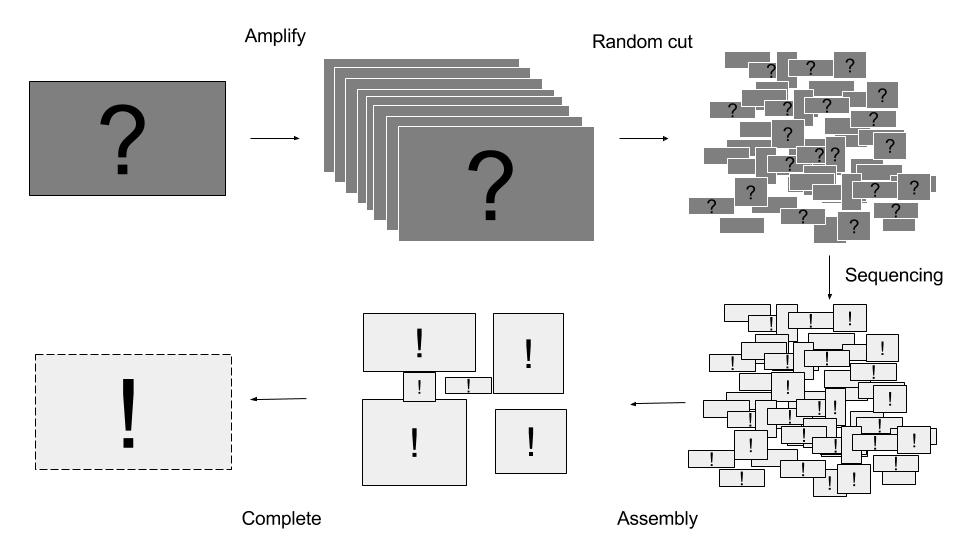
\includegraphics[height=.8\textheight]{figures/ass.jpg}  
%\end{center}
%\end{frame}
%%%%%%%%%%%%%%%%%%%%%%%%%%%%%%%%%%%%%%%%%%%%%%%%
%% \begin{frame}{DNA sequencing timeline}
%%  \begin{center}
%%  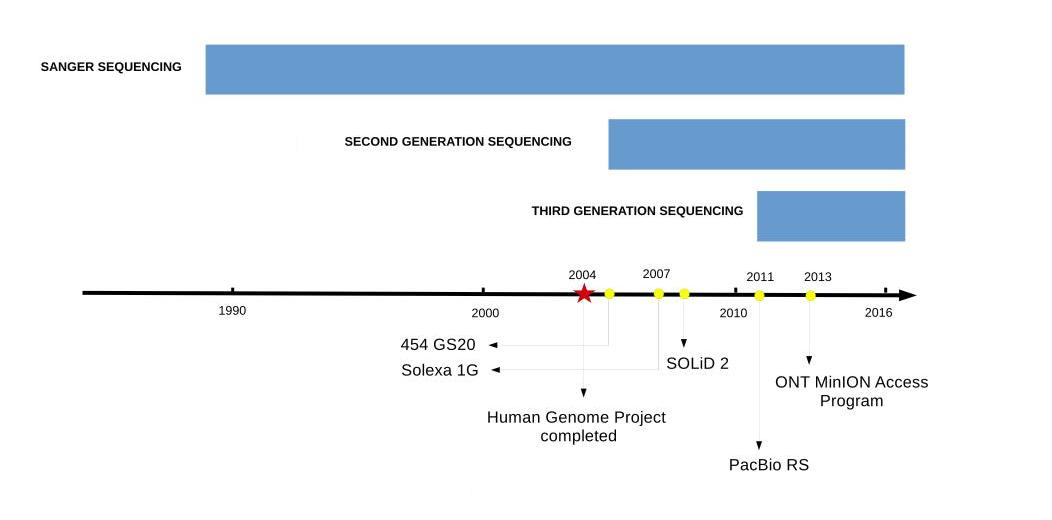
\includegraphics[width=\textwidth]{timeline.jpg}  
%% \end{center}
%% \end{frame}
%%%%%%%%%%%%%%%%%%%%%%%%%%%%%%%%%%%%%%%%%%%%%%%%
%\begin{frame}{Thesis project}
%\begin{itemize}
%\item Genome assemblies using only short-reads are usually fragmented.
%  \begin{itemize}
%  \item positional information are usually irretrievable
%  \item could be resolved by nanopore long-reads 
%  \end{itemize} 
%\item[$\Rightarrow$] complete the genome with lowest cost possible
%\item Existing assemblers can only work after sequencing has completed
%  \begin{itemize}
%  \item over-sequencing
%  \item	under-sequencing
%  \end{itemize} 
%\item[$\Rightarrow$] real-time assembly is desired
%\end{itemize}
%\end{frame}
%%%%%%%%%%%%%%%%%%%%%%%%%%%%%%%%%%%%%%%%%%%%%%%%
{
\setbeamertemplate{navigation symbols}{}
\setbeamertemplate{background canvas}{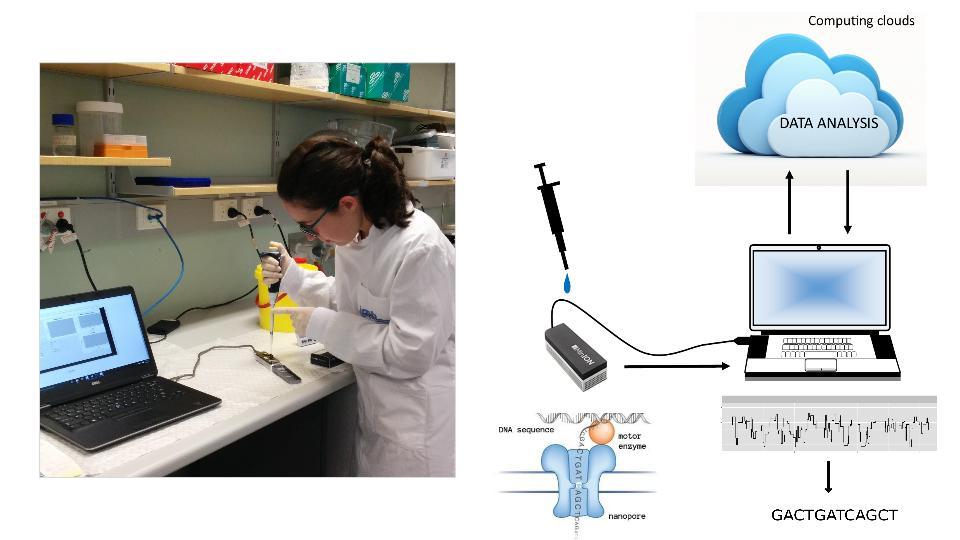
\includegraphics[width = \paperwidth]{figures/nanopore.jpg}}
\begin{frame}[plain]
\end{frame}
}
%
%{
%\setbeamertemplate{navigation symbols}{}
%\setbeamertemplate{background canvas}{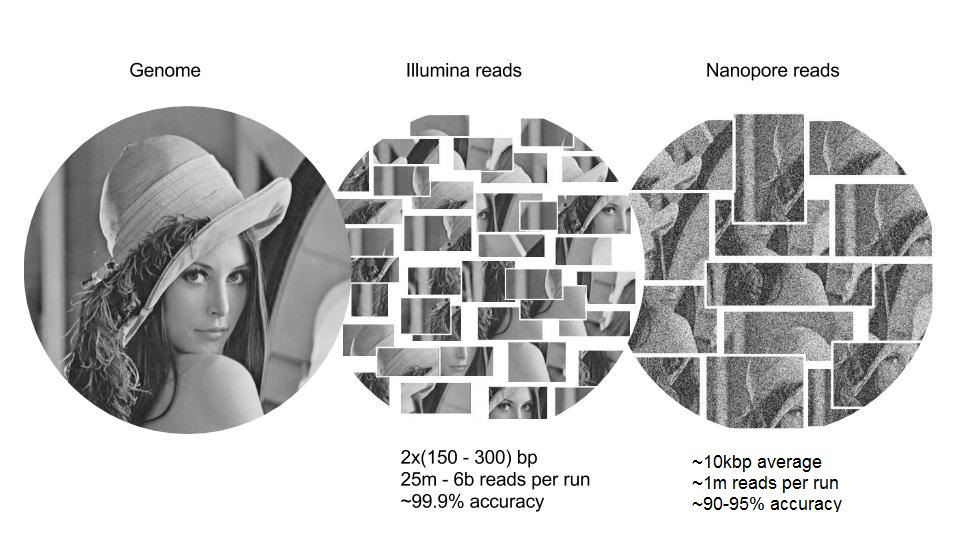
\includegraphics[width = \paperwidth]{figures/lena.jpg}}
%\begin{frame}[plain]
%\end{frame}
%}
%%%%%%%%%%%%%%%%%%%%%%%%%%%%%%%%%%%%%%%%%%%%%%%
\begin{frame}{Real-time analysis using Nanopore streaming data}
  \begin{center}
  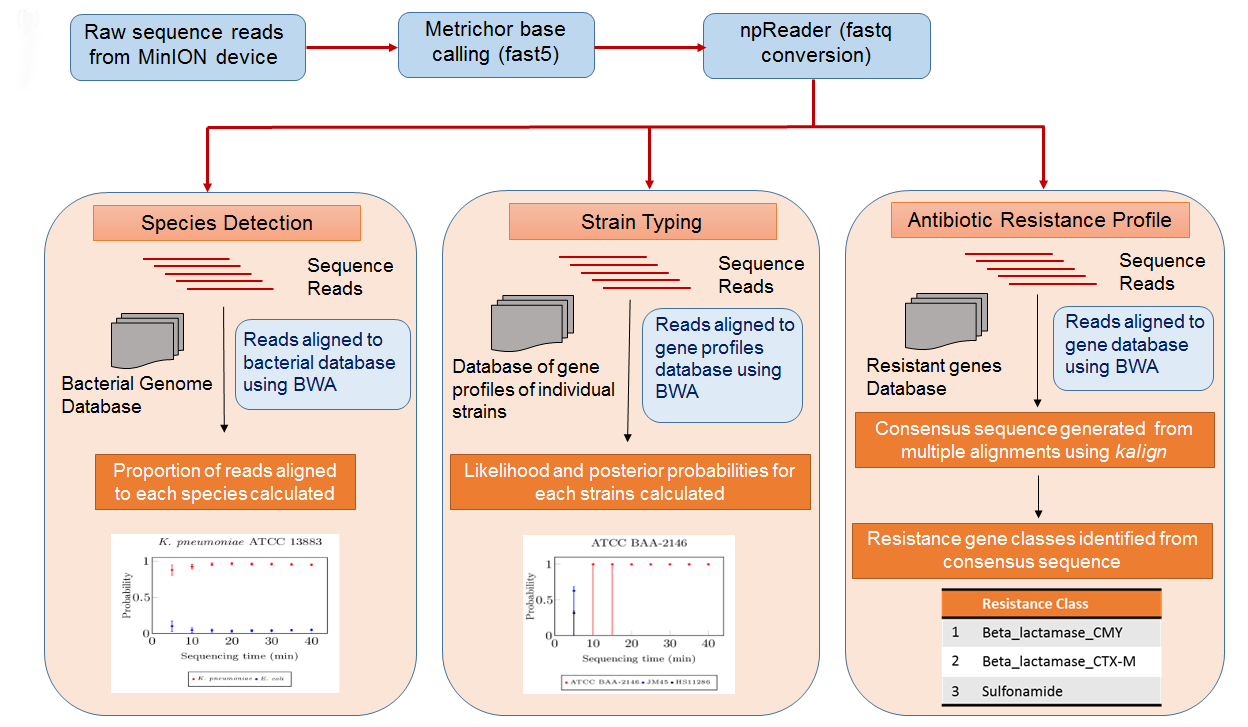
\includegraphics[width=0.6\textwidth]{realtime.jpg}  
   
 \vspace*{0.3cm}
Cao et al, 2016. DOI:10.1186/s13742-016-0137-2
 \end{center}
\end{frame}
%%%%%%%%%%%%%%%%%%%%%%%%%%%%%%%%%%%%%%%%%%%%%%%
%%%%%%%%%%%%%%%%%%%%%%%%%%%%%%%%%%%%%%%%%%%%%%%
\section{Real-time scaffolding microbial genomes}
%%%%%%%%%%%%%%%%%%%%%%%%%%%%%%%%%%%%%%%%%%%%%%%
%%%%%%%%%%%%%%%%%%%%%%%%%%%%%%%%%%%%%%%%%%%%%%%
% emphasis the STREAMING
\begin{frame}{\emph{npScarf} -- scaffold and complete genome assemblies}
 \begin{center}
 \vspace*{-0.6cm}
 \includegraphics[width=0.6\textwidth]{workflow.pdf}  
 
 \vspace*{-0.3cm}
Cao, Nguyen et al, 2017.  DOI:10.1038/ncomms14515
\end{center}
\end{frame}
%%%%%%%%%%%%%%%%%%%%%%%%%%%%%%%%%%%%%%%%%%%%%%%
%%%%%%%%%%%%%%%%%%%%%%%%%%%%%%%%%%%%%%%%%%%%%%%
% mention amount of data needed to complete kp2146
% compared with other method which use all of data
\begin{frame}{Scaffolding and completing genome results} 
\hspace*{0.25cm}
\vspace*{-.5cm}
 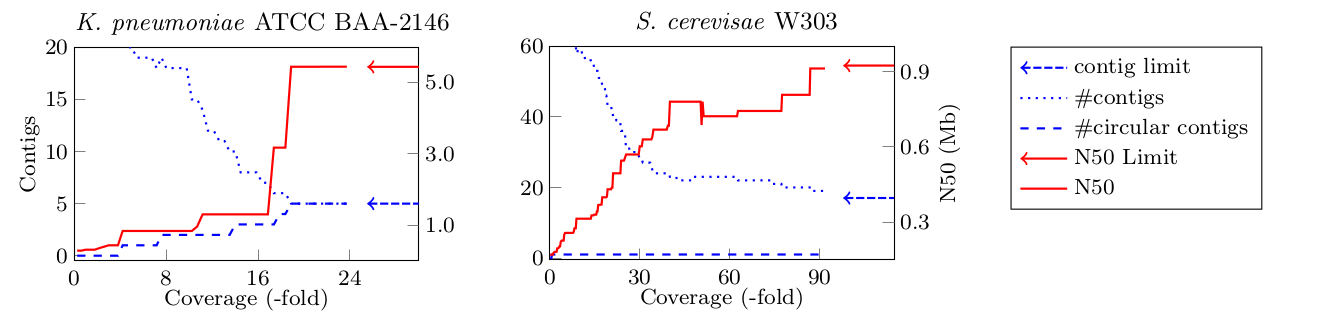
\includegraphics[width=.95\textwidth]{scaffold.png}  
 \onslide<1>
 \vspace*{.5cm}
 \medskip
 \\
\hspace{1cm} Genome size: 5.8Mb \hspace{1cm} Genome size: 12Mb
 \vspace*{-.5cm}
 \onslide<2>
\definecolor{Gray}{gray}{0.9}
\newcommand*\rot{\rotatebox{75}}
\setlength{\tabcolsep}{4pt}
\hspace*{-0.25cm}
\begin{tiny}
\begin{tabular}{lrrrrrrrrrrrrrr}
\cline{2-6}
\cline{9-13}

\cline{2-6}
\cline{9-13}

\centercell{\rot{Methods}}
& \centercell{\rot{\#Contig}} & \centercell{\rot{N50 (Mb)}} & \centercell{\rot{Mis-}\rot{assemblies}} & \centercell{\rot{Errors} \rot{/100Kb}} & \centercell{\rot{CPUhrs}} & &
& \centercell{\rot{\#Contig}} & \centercell{\rot{N50 (Mb)}} & \centercell{\rot{Mis-}\rot{assemblies}} & \centercell{\rot{Errors} \rot{/100Kb}} & \centercell{\rot{CPUhrs}}  
\\      
\cline{2-6} 
\cline{9-13}
\\
  \rowcolor{Gray}
  SPAdes  & 90 & 0.28 &  0 & 4.7 & 15.6 & &  & 364& 0.16 & 29 & 124.1 & 20.5  \\  
  -Hybrid & 17 & 3.10 & 1  & 6.6 & 16.1 & &  & 240& 0.35 & 68 & 158.1 & 67.8 \\
  -SSPACE & 53 & 0.40 & 4  &12.7 & 17.9 & &  & 263& 0.39 & 89 & 136.7 & 52.0 \\          
  -LINK   & 31 & 0.55 & 5  &16.1 & 19.7  & &  & 161& 0.58 & 83 & 143.0 & 47.5 \\
  \rowcolor{yellow!30}
  -npScarf& 5  & 5.40 & 0  &20.0 & 17.2  & & &  19 & 0.91 & 82 & 141.9 & 41.8 \\ 
  NaS     & 29 & 0.34 & 15 &18.9 & 328  & & & 121 & 0.15 & 123 & 140.1 & 9951 \\
  Nanocorr& 68 & 0.14 & 8  &141.3& 314  & &  & 108  & 0.60 & 133 & 197.0 & 7480 \\
  \hline
 \end{tabular}
 \end{tiny}
\end{frame}

%%%%%%%%%%%%%%%%%%%%%%%%%%%%%%%%%%%%%%%%%%%%%%%
\begin{frame}{\emph{npBarcode} -- demultiplexing nanopore reads in real time}
%\begin{center}
%\animategraphics[loop,autoplay,height=.75\textheight]{12}{animations/npreader/npreader-}{0}{300}
%\end{center}
\end{frame}

%%%%%%%%%%%%%%%%%%%%%%%%%%%%%%%%%%%%%%%%%%%%%%%
\begin{frame}{\emph{npBarcode} $\vert$ \emph{npScarf}}
\begin{figure}[!hpb]
\centering
\subcaptionbox{GN\_092}{\includegraphics[width=0.25\textwidth]{figures/s092.pdf}}%
\hfill
\subcaptionbox{GN\_096}{\includegraphics[width=0.25\textwidth]{figures/s096.pdf}}%
\hfill
\subcaptionbox{GN\_106}{\includegraphics[width=0.25\textwidth]{figures/s106.pdf}}%
\hfill
\subcaptionbox{GN\_133}{\includegraphics[width=0.25\textwidth]{figures/s133.pdf}}%
\end{figure}
\vspace*{-0.3cm}
Nguyen et al 2017.  DOI:10.1093/bioinformatics/btx537
\end{frame}
%%%%%%%%%%%%%%%%%%%%%%%%%%%%%%%%%%%%%%%%%%%%%%%
\section{Real-time assembly with assembly graph}
%%%%%%%%%%%%%%%%%%%%%%%%%%%%%%%%%%%%%%%%%%%%%%%
%%%%%%%%%%%%%%%%%%%%%%%%%%%%%%%%%%%%%%%%%%%%%%%
%%%%%%%%%%%%%%%%%%%%%%%%%%%%%%%%%%%%%%%%%%%%%%%%%
\begin{frame}{Microbial genome finishing on assembly graph}
\begin{itemize}
\item \textbf{Advantages}
  \begin{itemize}
  \item Higher quality assembly by reducing gaps.
  \item Decrease mis-assemblies from alignment-based scaffolding
  \end{itemize} 
\item \textbf{Challenges}
  \begin{itemize}
  \item More computational expensive: graph traversing \& path finding
  \item	How to adapt to real-time fashion?
  \end{itemize} 
\end{itemize}
\end{frame}
%%%%%%%%%%%%%%%%%%%%%%%%%%%%%%%%%%%%%%%%%%%%%%%%%
\begin{frame}{\emph{Unicycler}'s hybrid assembly pipeline}
\begin{itemize}
\item SPAdes k-mer optimization to reduce dead-ends
\item Using long reads to guide graph traversal
\end{itemize}
\begin{figure}[!hpb]
\centering
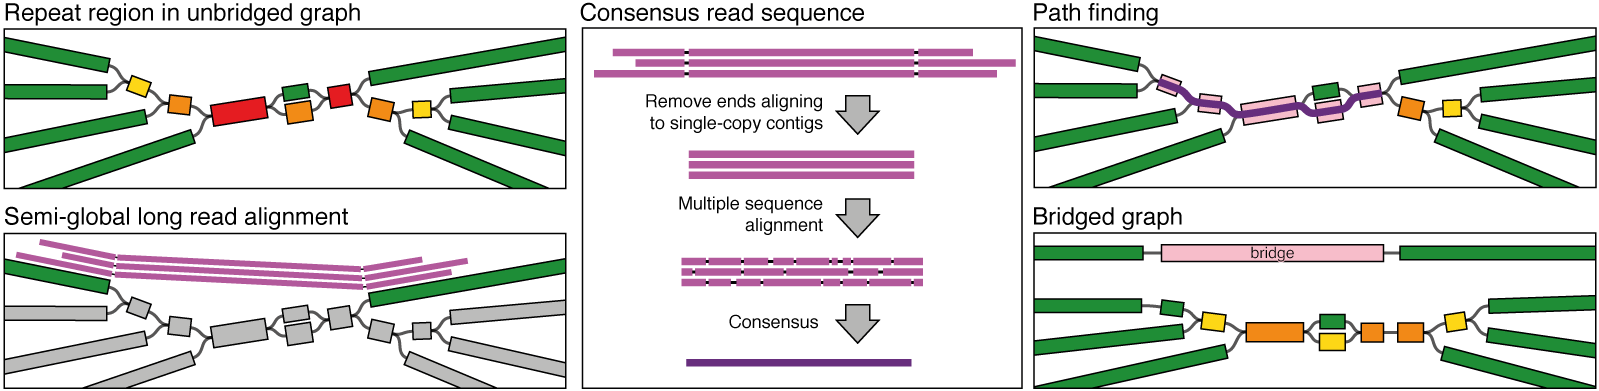
\includegraphics[width=.9\textwidth]{long_read_bridging.png}
\end{figure}
\vspace*{-0.3cm}
Wick et al 2017.  DOI:10.1371/journal.pcbi.1005595
\end{frame}
%%%%%%%%%%%%%%%%%%%%%%%%%%%%%%%%%%%%%%%%%%%%%%%%%
\begin{frame}{\emph{npGraph}: real-time assembly graph resolver}
\emph{\textbf{Pipeline:}}
\begin{enumerate}
  \item Graph preprocessing
  \begin{itemize}
    \item cluster graph nodes into different bins
    \item estimate multiplicity for graph components
  \end{itemize}
  \item Resolve graph in real-time
  \begin{itemize}
  	\item use long reads to bridge unique nodes (contigs)
  	\item clean and simplify graph
  \end{itemize}
\end{enumerate}
\end{frame}
%%%%%%%%%%%%%%%%%%%%%%%%%%%%%%%%%%%%%%%%%%%%%%%%%
%%%%%%%%%%%%%%%%%%%%%%%%%%%%%%%%%%%%%%%%%%%%%%%%%
\begin{frame}{Binning contigs}
\begin{itemize}
	\item MetaVelvet: length-weighted kmer frequency distribution
		\begin{figure}[!hpb]
		\centering
		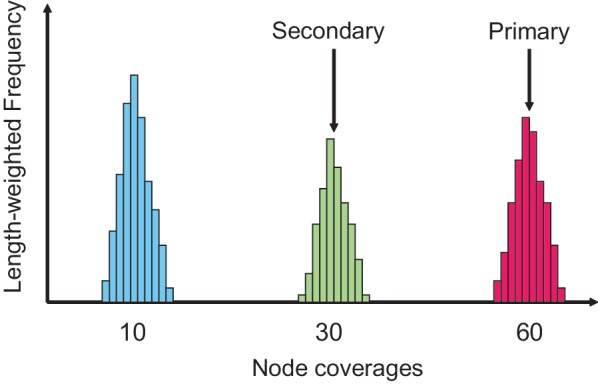
\includegraphics[width=.45\textwidth]{figures/metavelvet.jpg}
		\end{figure}
	\item Using external tools: metabat2, maxbin.
\end{itemize}
\end{frame}
%%%%%%%%%%%%%%%%%%%%%%%%%%%%%%%%%%%%%%%%%%%%%%%%%
%%%%%%%%%%%%%%%%%%%%%%%%%%%%%%%%%%%%%%%%%%%%%%%%%
\begin{frame}{Bridging contigs}
\begin{center}
 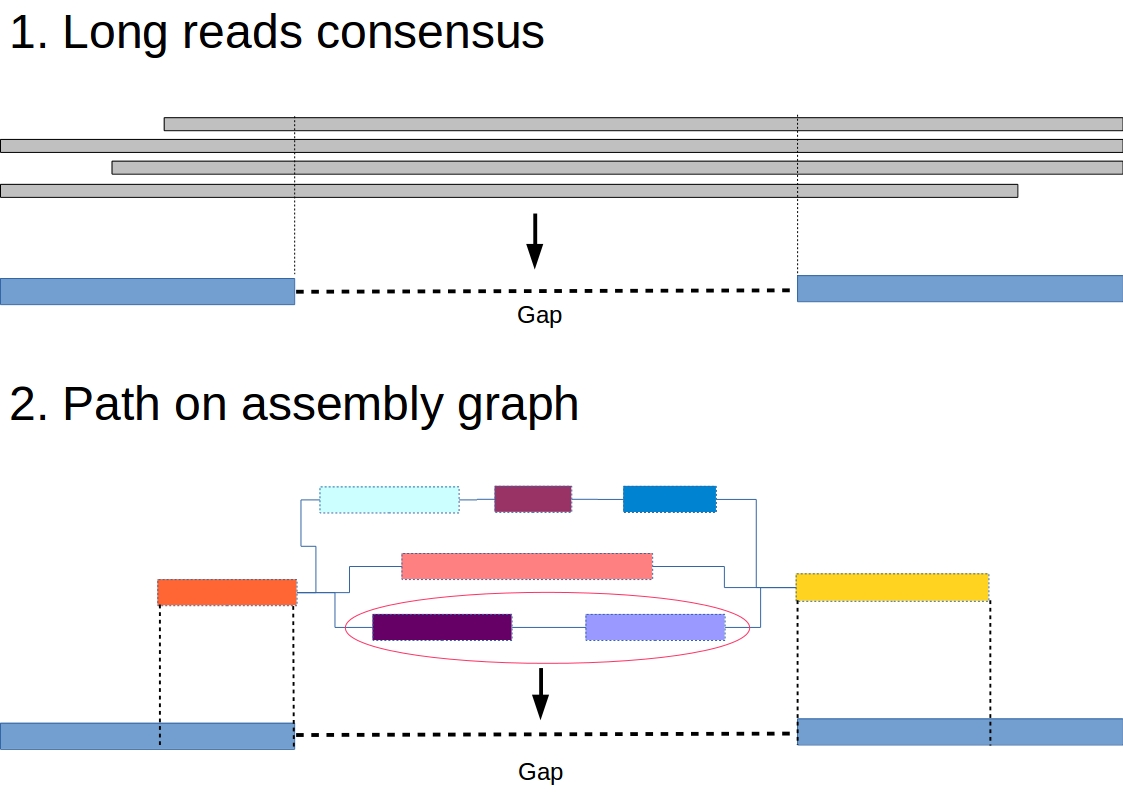
\includegraphics[height=.8\textheight]{gapfilling.jpg}  
\end{center}
\end{frame}
%%%%%%%%%%%%%%%%%%%%%%%%%%%%%%%%%%%%%%%%%%%%%%%%%
\begin{frame}{Graph resolving}
\begin{center}
 \includegraphics[height=.7\textheight]{figures/bridge_merging.pdf}  
\end{center}
\end{frame}
%%%%%%%%%%%%%%%%%%%%%%%%%%%%%%%%%%%%%%%%%%%%%%%%%
\begin{frame}{\emph{npGraph} GUI}
%\begin{center} 
%	\animategraphics[loop,autoplay,width=.8\textwidth]{12}{animations/npgraph/npgraph-}{0}{400}
%\end{center}
\end{frame}
%%%%%%%%%%%%%%%%%%%%%%%%%%%%%%%%%%%%%%%%%%%%%%%
\begin{frame}{\emph{npGraph} on microbial isolates}
%\begin{figure}[!hpb]
%\centering
%\animategraphics[autoplay,height=.4\textheight]{20}{animations/kp_ntuh/images_}{00001}{00327}
%~
%\animategraphics[autoplay,height=.4\textheight]{20}{animations/ab30/images_}{00001}{00350}
%\\ \vfill
%\animategraphics[autoplay,height=.4\textheight]{20}{animations/kp_mgh/images_}{00001}{00336}
%~
%\animategraphics[autoplay,height=.4\textheight]{20}{animations/shigella/images_}{00001}{00400}
%\end{figure}
\end{frame}
%%%%%%%%%%%%%%%%%%%%%%%%%%%%%%%%%%%%%%%%%%%%%%%
%%%%%%%%%%%%%%%%%%%%%%%%%%%%%%%%%%%%%%%%%%%%%%%
\begin{frame}{\emph{npGraph} on metagenomics mock communities}
%\begin{figure}[!hpb]
%\subcaptionbox{Zymo Even}{\animategraphics[autoplay,width=.48\textwidth]{12}{animations/zymoeven/images_}{00001}{00600}}%
%\hfill
%\subcaptionbox{Zymo Log}{\animategraphics[autoplay,width=.48\textwidth]{12}{animations/zymolog/images_}{00050}{00650}}%
%\end{figure}
\end{frame}
%%%%%%%%%%%%%%%%%%%%%%%%%%%%%%%%%%%%%%%%%%%%%%%
\begin{frame}{Issues}
\begin{itemize}
\item DBG assembly graph quality and pre-processing is important 
	\begin{itemize}
		\item high Illumina sequencing coverage
		\item binning \& multiplicity estimation
	\end{itemize}
\item Nanopore data is used for bridging only
\end{itemize}
\end{frame}
%%%%%%%%%%%%%%%%%%%%%%%%%%%%%%%%%%%%%%%%%%%%%%%
%%%%%%%%%%%%%%%%%%%%%%%%%%%%%%%%%%%%%%%%%%%%%%%
%%%%%%%%%%%%%%%%%%%%%%%%%%%%%%%%%%%%%%%%%%%%%%%
%%%%%%%%%%%%%%%%%%%%%%%%%%%%%%%%%%%%%%%%%%%%%%%
{
\setbeamertemplate{navigation symbols}{}
\setbeamertemplate{background canvas}{\includegraphics[width = \paperwidth]{figures/group.jpg}}
\begin{frame}[plain]
\end{frame}
}

\end{document}
